\chapter{Appendix: Managing Rosetta datasets with SQL}

\section{Introduction}

Screening small molecule libraries with RosettaHTS requires the generation of very large number of models. 
For example, a screen of 250,000 compounds will result in 50,000,000 generated Rosetta models.
Because RosettaHTS only needs the top 1 model generated for each ligand, 99.995\% of this data will not be needed.
To avoid unnecessarily storing data, RosettaHTS stores generated models in a relational database.
Here  the technical details of the database storage framework used by RosettaHTS are described.
This framework was developed collaboratively by myself, Chris Miles at the University of Washington, Matt O'Meara at the University of North Carolina, and Tim Jacobs at the University of North Carolina, all of whom contributed equally to the project. 

\section{Features reporter architecture}

The data storage framework used by RosettaHTS is a subset of a statistical analysis framework within Rosetta called the Features Reporter.
The Features Reporter framework consists of an \ac{ORM} that allows \ac{SQL} schema definitions, queries and insertion statements to be composed in C++, and a reporting system used for computing statistical data and storing it in the database.
The \ac{ORM} was developed using CppDB(http://cppcms.com/sql/cppdb/) \ac{SQL} library, which allows the features reporter to work with SQLite, MySQL and Postgres database backends.
As all 3 of these back ends have different caveats, behaviors and syntax idioms, the \ac{ORM} is responsible for constructing the appropriate MySQL command and sending it to the server.

In addition to allowing for the transparent support of multiple Database Backends, the \ac{ORM} system makes it possible for a C++ programmer to easily define new \ac{SQL} objects without being familiar with \ac{SQL} syntax. 
For example, the C++ code reproduced below defines an \ac{SQL} table containing structure ID, residue number, 3 letter residue name, and residue type fields, then generate the appropriate \ac{SQL} syntax to create this table, and execute the \ac{SQL} command on the database server.

\singlespace
\begin{Verbatim}
Column struct_id("struct_id", new DbBigInt(), false);
Column resNum("resNum", new DbInteger(), false);
Column name3("name3", new DbText(), false);
Column res_type("res_type", new DbText(), false);

utility::vector1<Column> residues_pkey_cols;
residues_pkey_cols.push_back(struct_id);
residues_pkey_cols.push_back(resNum);

Schema residues("residues", PrimaryKey(residues_pkey_cols));
residues.add_column(struct_id);
residues.add_column(resNum);
residues.add_column(name3);
residues.add_column(res_type);
residues.add_foreign_key(
  ForeignKey(struct_id, "structures", "struct_id", true));

residues.write(db_session);
\end{Verbatim}
\doublespace

This model of database interaction allows multiple database systems to be supported with a single code base, which is critical given the diversity of hardware and software operated by Rosetta users.
Additionally, it allows support to be added for additional database systems without any change to the code defining feature tables. 

The Features Reporter has been previously described in the literature \citep{LeaverFay:2013fn} as a method for collecting and analyzing statistics from large numbers of Rosetta models.  
In the sections below we will describe the specific application and usage of this framework for the storage and retrieval of protein models in a high throughput screening environment. 

\section{Pose storage schema}

RosettaHTS uses a subset of the Features Reporter system to store and retrieve protein structure information from the database.
In the most simple case, it would be possible to store only the atom and residue names, chain information, and cartesian coordinates for each atom, and effectively replicate the information present in a \ac{PDB} file.
However, storing this limited subset of information requires that Rosetta rebuild the internal data-structures representing the protein structure every time the pose is loaded, as is done when taking input from a \ac{PDB} file.
While this is normally acceptable, in rare cases, there are multiple correct configurations that these data structures can take on, and thus, recomputing them can result in a slightly different input model, and numeric inconsistencies in scoring across multiple loads of the structure.
While these  numeric inconsistencies do not typically lead to scientific inconsistencies, their presence can complicate data analysis.

In order to rectify this problem, the RosettaHTS pose storage schema stores not only the information reflected in the protein \ac{PDB} file, but also all of the derived data created by Rosetta.
The storage of this information makes it possible to precisely store and recover the protein structure as it is internally represented by Rosetta.
The Pose storage schema is illustrated in Figure \ref{fig:pose_schema}.  Each block in the figure represents an \ac{SQL} table storing a subset of 
of the information needed to reconstruct the pose.
Connections between the blocks indicate "Relationships" between the tables.  Connecting the tables with relationships makes it possible to link data elements that related to each other, while simultaneously allowing for Pose data to be queried efficiently.

\begin{figure}
%figure 2 in orginal paper
\centering
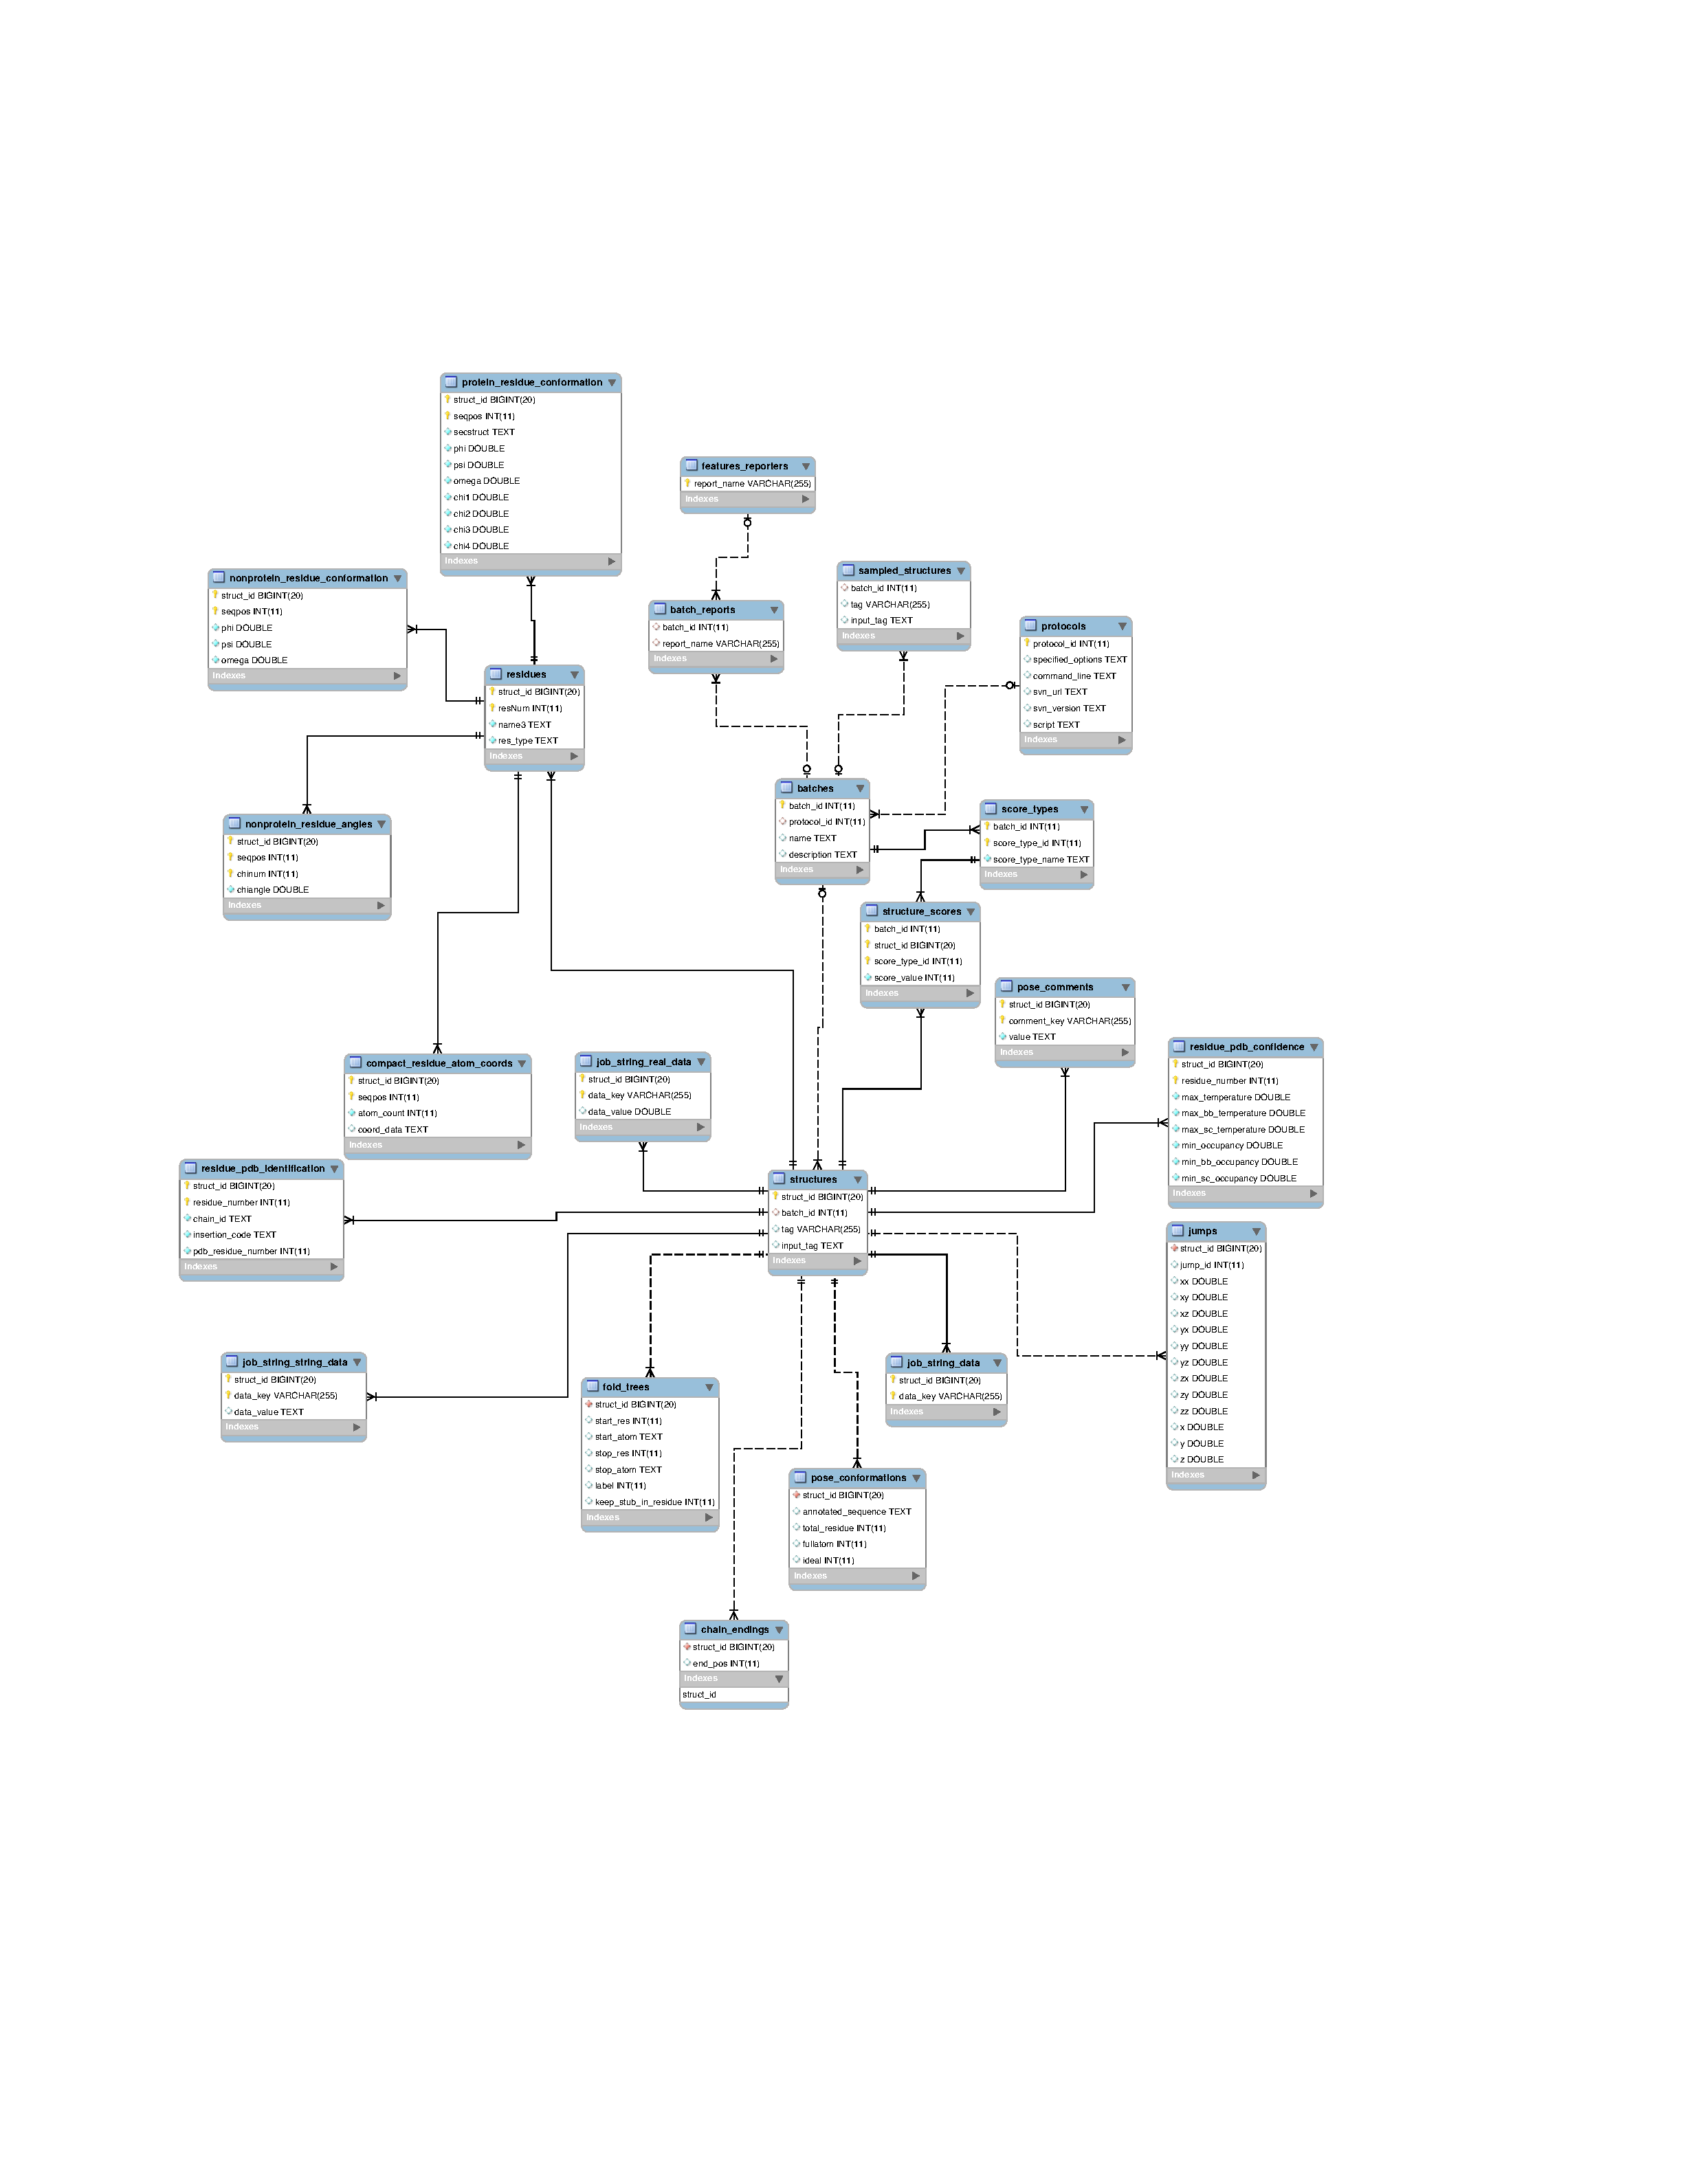
\includegraphics[width=6in]{figures/mysql/mysql_model.pdf}
\caption{
A schematic representation of the information stored by the RosettaHTS pose schema
}
\label{fig:pose_schema}
\end{figure}

A critical component of the design of a relational database schema is a means of uniquely identifying models.
In this case, uniqueness from the point of view of the database has a different meaning than biochemical uniqueness.
If Rosetta is run twice with the same protocol and produces two absolutely identical output models, those models should be stored separately in the database and given unique identifiers, even though they contain the same information. 
Additionally, given a specific stored Pose, it should be possible to identify which execution of the Rosetta application resulted in that Pose, and at what point in the overall protocol the Pose (or other statistical data) was generated. 
To accomplish this, the identification of structures is handled with a three tiered structure.
The top tier is the "Protocol" level.
A new Protocol is generated every time a Rosetta process outputs to a database.
Each protocol has a unique number identifying it which is assigned by the database server.
The Protocol stores the version of Rosetta that was used, as well as the command line options and XML script specified by the user.
Each Protocol can generate one or more "Batch" which is the second level of the identification system.
A Batch is generated every time a Protocol outputs structural data. If RosettaHTS is only outputting completed protein models, only one batch exists per protocol.
If the Features Reporter is also being used in the middle of the protocol to generate extra statistics, additional batches will be generated. 
Each Batch has a unique number identifying it, and references the protocol that was responsible for creating it.
The last tier in the identification system is the "Structure".
A new structure is generated every time Rosetta produces a model.
Each structure has a unique number identifying it, and references the batch that resulted in the creation of that structure.
Additionally, each structure record has a human readable "tag" describing its output, and references the input structure that was used as a basis for the model. 
In this way, the batch, protocol and structure tables can be joined by their related IDs such that, given a structure stored in the database, one can determine precisely what Rosetta command was used to generate that structure, and at what point in the Rosetta protocol the structure was generated. 

The Structure ID described above is used as the central unique identifier, and all the information associated with an individual model is related using this ID.

The RosettaHTS database IO schema stores the following information:

\begin{itemize}
	\item Text and numeric comment data that some Rosetta components insert in a pose for scoring and tagging purposes during the protocol.
	\item The range of B-factors for atoms in each residue.
	\item The "Jumps" in the structure.  Jumps are data structures which represent the spatial relationship between protein chains as a Rotation and Translation matrix.
	\item The sequence associated with the structure, annotated with the identity of any non-canonical, modified or ligand residues.
	\item The ending position of each chain.
	\item The "Fold Tree" defining the structure.  The Fold tree is a data structure used by Rosetta to describe how different parts of the protein are related in space.  Fold Trees can be configured to make it possible to rapidly perturb large parts of the protein as a rigid body.  DiMaio et al. \citep{DiMaio:2011cu} provides an example of a fold tree manipulation in practice.
	\item The Chain ID, insertion code, and residue number present in the original PDB file
	\item The values of each energy term in the score function when the structure was last scored.
	\item The cartesian coordinates of each atom.
	\item The chi angles of each canonical amino acid.
	\item The rotation angles of each non-canonical amino acid or non-protein molecule.
\end{itemize}

In addition to providing infrastructure for outputting Rosetta models, the RosettaHTS pose IO schema provides infrastructure for using this data as input into Rosetta.
Both output to and input from the database is handled by the Rosetta job distribution system.
This means that any Rosetta application can use a database as a data storage mechanism, without any additional programming on the part of the developer of the application.
Furthermore, because the same database can be used for both output and input simultaneously, a Rosetta modeling protocol that relies on different applications being used in different stages can use the database for data management at each stage.

\section{Database Filters}

Historically, Rosetta applications have considered each model independently of each model.
This is primarily an engineering decision.
If each model is considered independently, it means that only the current structure needs to be stored in memory, reducing system resource requirements. 
Additionally, if each model is considered independently, the design of Rosetta is simpler, as it each module of the code does not need to consider the accumulation of state between jobs.
However, while this decision was critical to making Rosetta a maintainable piece of software, it has severely limited the ability to perform filtering and output of models. 
Specifically, filters could historically be created only based on single protein metrics.
A filter could, for example, output models with a score lower than a certain fixed cutoff, or that had a degree of packing better than a cutoff.
However, in the case of protein-ligand docking, we are unable to set fixed score cutoffs, as the range of scores seen will vary from ligand to ligand.
The preferred means of filtering ligand models is to accept the lowest scoring model generated for each protein-ligand pair.
This type of filter cannot be created with the traditional Rosetta filter system, requiring that all models be output, and filtered after the fact.
The RosettaHTS docking protocol requires that 200 models be generated per protein-ligand pair. 
Given that each compressed model requires approximately 90 kilobytes of storage space, the total requirement per protein-ligand pair is roughly 18 megabytes.
Thus, a 250,000 compound screen would require about 4.5 terabytes of compressed storage space. 
The infrastructure required to store and analyze a dataset of this size outstrips the abilities of most research groups, and the storage of the complete dataset is particularly senseless as nearly all of it will be deleted after the initial round of filtering. 

The Database Filter system leverages the properties of the \ac{SQL} database system to make it possible for the first time to create Rosetta filters which take into account the context of previously generated models.
\ac{SQL} is designed to conduct rapid queries of stored data, and as these queries are conducted by the database engine itself, rather than Rosetta, the operation of the filter does not require that state be kept between Rosetta jobs and does not result in additional memory requirements.

A Rosetta Database Filter can have 3 possible outcomes:  The current model is not output, the current model is output, or the current model replaces an existing model.
To accomplish this the Database Filter conducts a query of the existing structures in the database  to identify if the current model is suitable to be output, and to identify the model that it will replace if necessary. 
Currently, filters exist to filter models by the top percent or top count by score.
The creation of additional filters can be accomplished by the implementation of a new DatabaseFilter class with a single method.
While the current usage for filtering by score percentile is relatively simple, the Database Filter framework could hypothetically be used to implement histogram matching filters or other filters requiring deep analysis of the existing dataset.
This would be effectively impossible in the context of the classical Rosetta filtering system, but relatively trivial with a Database Filter.

\section{Performance Considerations and Selection of a Database backends}

Currently, the Rosetta database system supports three different database back ends.
The selection of the appropriate back end is an important consideration, and will depend largely on the way in which the database will be used.

\subsection{SQLite3}
SQLite3 (https://www.sqlite.org/) is the default option for Rosetta database support.
SQLite3 stores the entire database as a single binary file, and the database engine itself is built into Rosetta.
The primary advantage of using SQLite3 is that it requires no additional hardware or software infrastructure, which makes it idea for prototyping a protocol or handling small "one-off" analysis of data.
SQLite3 was designed to be used explicitly with single threaded applications, this means that only a single Rosetta process at a time can write to an SQLite database.
Additionally, SQLite3 produces a very large number of random access operations to the filesystem.
The nature of these operations is such that heavy usage of SQLite3 can severely degenerate the performance of a network file system.
For this reason, we recommend that SQLite3 only be used only with local disks, and preferably with Solid State Drives rather than traditional "Spinning" disks.
Despite these limitations, Rosetta protocols requiring large amounts of memory and complex statistical analysis can be performed very efficiently using SQLite3.
The majority of the data collection and analysis described in Leaver-Fay et al. \citep{LeaverFay:2013fn} was conducted using an SQLite3 database.

\subsection{PostgreSQL and MySQL}

PostgreSQL (http://www.postgresql.org/) and MySQL (http://www.mysql.com/) are freely available server based SQL solutions.
In both cases, an independent server is used, and Rosetta communicates with this server over the network.
The details of the installation and configuration of these systems are beyond the scope of this document, however either piece of software is acceptable for use with RosettaHTS. 
For large scale data operations, PostgreSQL and MySQL have substantial advantages over SQLite3. 
In both cases, many processes can simultaneously write to a single database, and the database server ensures that data is written correctly even for large numbers of concurrent reads and writes.
Additionally, the use of a server based SQL solution offloads the computational and IO complexity involved with reading from and writing to the database to a separate machine than the one running Rosetta.
This separation of work can have a substantial performance benefit.
It is possible to create a Rosetta protocol which produces database requests that outstrip the processing ability of even a reasonably powerful database server.
The precise nature of these limitations will depend on the Rosetta protocol, as well as the specific details not only of the database server software configuration but also the server and network infrastructure being used.
For this reason, we advise empirically determining the performance limitations and requirements of your specific protocol through benchmarking tests prior to large scale screening. 

\section{Storing and retrieving poses from the Rosetta command line}

Rosetta provides a set of command line options for storing and retrieving poses from a database.
These command line options can be used with any Rosetta application other than the "abinitio" application, and will function identically in any protocol.

\subsection{Connecting to a database}

Connecting to a Rosetta database depends on the type of database back end being used.  Regardless of what back end is being used, back end mode and the database name must be specified:

\singlespace
\begin{Verbatim}
-inout:dbms:mode <mode>
-inout:dbms:database_name <db_name>
\end{Verbatim}
\doublespace

where \texttt{<mode>} should be replaced by the database mode (either \texttt{mysql}, \texttt{sqlite} or \texttt{postgres}), and \texttt{<db\_name>} should be replaced by the name of the database file if using sqlite, the schema name if using MySQL, and the database name if using PostgreSQL.

If you are using MySQL or PostgreSQL as a back end, you must specify several additional options connect to the server

\singlespace
\begin{Verbatim}
-inout:dbms:host <host>
-inout:dbms:user <username>
-inout:dbms:password <password>
-inout:dbms:port <port>
\end{Verbatim}
\doublespace

Where \texttt{<host>} is the address of the database server, \texttt{<username>} is the username of a user with permission to read and write from the database, \texttt{<password>} is the password of that user, and \texttt{<port>} is the TCP port that the server is running on. 

Additionally, if you will be running RosettaHTS or any other protocol that results in very large numbers of structures being output to a single database (more than 100,000), the database should be configured to reduce the number of \texttt{INSERT} statements necessary to write a complete model.
This is accomplished by modifying the database storage schema to produce a single record per residue rather than a single record per atom.  This enormously reduces the storage and network bandwidth requirements at the cost of data analyzability, and should be considered a required setting when using RosettaHTS.
Compact schema mode is enabled with the following option:

\singlespace
\begin{Verbatim}
-inout:use_compact_residue_schema true
\end{Verbatim}
\doublespace

\subsection{Writing to database}

Once the database connection options above are specified, Rosetta can be configured to write all output models to the specified database with a single output option:

\singlespace
\begin{Verbatim}
-out:use_database
\end{Verbatim}
\doublespace

If the use of a Database Filter is desired, it should be specified with another option:

\singlespace
\begin{Verbatim}
-out:database_filter <filter_name> <score_term> <value>
\end{Verbatim}
\doublespace

Where \texttt{<filter\_name>} is the name of the database filter to use, \texttt{<score\_term>} is the name of the scoring term to filter by, and \texttt{<value>} is the cutoff value to use. 
At the time of writing, the following filters exist:

\begin{itemize}
	\item \texttt{TopPercentOfEachInput} -- Output models in the top $n\%$ of models for each input structures by specified score.
	The specified cutoff value should be a decimal between 0 and 1. 
	\item \texttt{TopPercentOfAllInputs} -- Output models in the top $n\%$ of models over all input structures by the specified score.
	The specified cutoff value should be a decimal between 0 and 1.
	\item \texttt{TopCountOfEachInput} -- Output the top $n$ models for each input structures by the specified score.
	The specified cutoff value should be an integer.
	\item \texttt{TopCountOfAllInputs} -- Output the top $n$ models over all input structures by the specified score.
	The specified cutoff value should be an integer.
\end{itemize}

\subsection{Reading from a database}

Rosetta can be configured to read input models from the specified database with a single input option:

\singlespace
\begin{Verbatim}
-in:use_database
\end{Verbatim}
\doublespace

Note that both \texttt{-in:use\_database} and \texttt{-out:use\_database} can be used simultaneously.
This is valuable in an interactive protocol, as the results from the current round of iteration can be written to the same database as the results from the previous round. 

It is frequently desirable to read only a subset of structures from a database. 
If the structure IDs of the desired structures are known they can be specified with the following command:

\singlespace
\begin{Verbatim}
-in:dbms:struct_ids <struct_id_list>
\end{Verbatim}
\doublespace

Where \texttt{<struct\_id\_list>} is a space separated list of structure IDs.

If the structure IDs are not known, it is possible to select a subset of the database using an \ac{SQL} select statement:

\singlespace
\begin{Verbatim}
-in:select_structures_from_database <statement>
\end{Verbatim}
\doublespace

where \texttt{<statement>} is an SQL statement that performs a \texttt{SELECT} operation that returns either a struct\_id or tag column from the database.  As a simple example, the statement:

\singlespace
\begin{Verbatim}
SELECT struct_id FROM job_string_real_data 
	WHERE data_key = "total_score" 
	ORDER BY data_value ASC LIMIT 500;
\end{Verbatim}
\doublespace

Would select the structure IDs of the 500 lowest scoring models by total score.
This command line option is potentially dangerous as minimal syntax validation is performed by Rosetta and the specified statement is executed on the \ac{SQL} server.
Make sure only to use this command line option with trusted user input, and do not expose any protocol that uses it as a web server.